\chapter{Descripción del Juego}

El \textit{Multi-Agent Programming Contest}\cite{BehrensAMAI2010b} (MAPC) es un
concurso de programación de Inteligencia Artificial iniciado en el año 2005, 
organizado por la Clausthal University of Technology 
\footnote{Más información \texttt{www.tu-clausthal.de}}, con el objetivo de 
estimular la investigación en el área de desarrollo y programación de 
Sistemas Multi-Agente. Para ello, la competencia propone diferentes 
escenarios de juego de manera anual, que obligan a los participantes tanto a 
identificar y resolver problemas clave, como a explorar lenguajes, 
plataformas y herramientas de programación para Sistemas Multi-Agente.

La organización entrega a los participantes de los ejecutables y documentación
necesarios para el correcto diseño, desarrollo y testeo de los sistemas 
implementados. Se cuenta con el servidor \textit{MASSim}, el cual se conecta
con los agentes a través de \textit{sockets}, y de la misma manera lo hace con
el monitor. Este último ofrece una interfaz gráfica (Fig. \ref{fig:ssjuego}), 
a través de la cual se puede observar el movimiento de los agentes, entre 
otros.

\begin{figure}
\centering
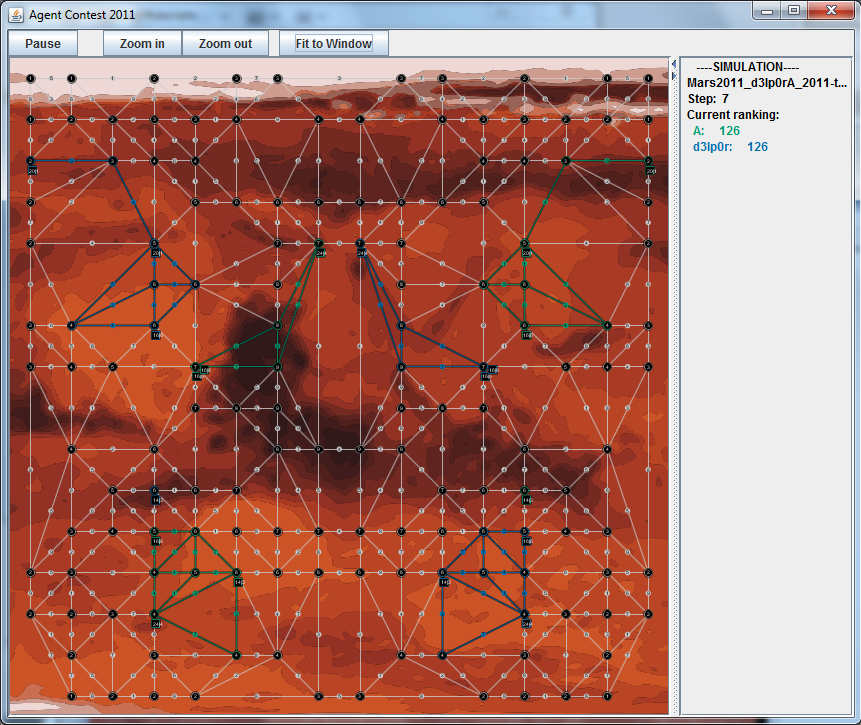
\includegraphics[width=\textwidth]{ssjuego.png}
\caption{Captura de pantalla de la interfaz gráfica del monitor del servidor.}
\label{fig:ssjuego}
\end{figure}

\section{Escenario}

El escenario del año 2011 está formado por el mapa de un planeta representado 
mediante un grafo. Cada vértice del grafo es una locación válida (y tiene un 
valor determinado), y existen arcos (con diferente costo de energía) que 
permiten a un agente desplazarse de una locación a otra. Un mapa del estilo
al usado durante la competencia se puede observar en la Fig. \ref{fig:ssjuego}.
Uno más reducido se puede encontrar en la Fig. \ref{fig:ssmapa}.

\begin{figure}
\centering
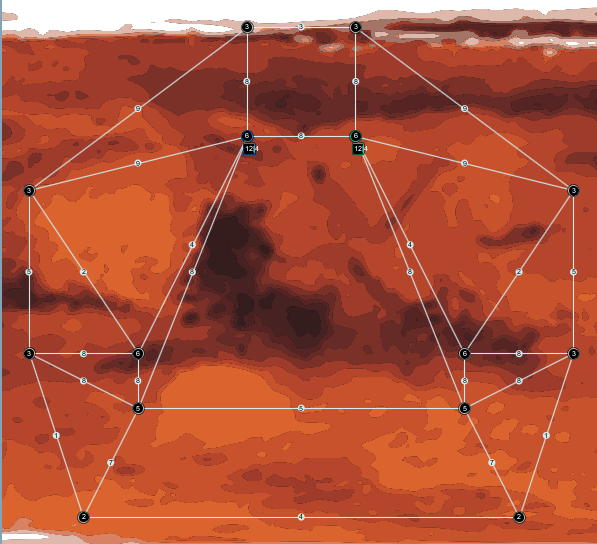
\includegraphics[width=\textwidth]{ssmapa.png}
\caption{Captura de pantalla de un mapa de tamaño reducido.}
\label{fig:ssmapa}
\end{figure}


En cada ronda de la competición participan dos equipos rivales. Cada equipo 
posee un conjunto de agentes con diferentes roles preestablecidos 
(\textit{Explorador}, \textit{Saboteador}, \textit{Reparador}, 
\textit{Sentinela} e \textit{Inspector}). El rol de cada agente define tanto 
el conjunto de acciones que puede realizar, como sus características físicas
(\textit{Energía}, \textit{Salud}, \textit{Fuerza} y \textit{Rango de Visión}).

\section{Puntaje}

La simulación del juego se desarrolla por turnos, y en cada turno se otorga 
a los equipos una determinada cantidad de puntos según el estado de la 
simulación. El objetivo del juego es obtener la mayor cantidad de puntos 
posibles cuando la simulación termina.

Para obtener puntos, los agentes de cada uno de los equipos deben lograr 
formar \textit{``zonas''} en el mapa logrando posicionarse en diferentes 
locaciones de manera estratégica. La predominancia de un equipo sobre el 
otro en los nodos es determinada por un algoritmo bien definido para la 
competencia, y el valor de todos los nodos dominados por un equipo es el 
principal factor del puntaje otorgado en cada uno de los turnos de la 
simulación. Algunas otras situaciones, como el logro de determinados 
\textit{achievements}, pueden otorgar puntos adicionales al equipo.

\section{Acciones}

Todos los agentes tienen acciones en común que pueden realizar en cada uno 
de los turnos de la simulación:

\begin{itemize}
	\item \texttt{goto(X)}: el agente se desplaza hacia el nodo X, siempre 
    y cuando exista un arco que conecte el nodo actual del agente con X, y 
    dicho arco tenga un costo menor a la energía actual del agente.
	\item \texttt{survey(X)}: el agente recibe en su próxima percepción los 
    costos de todos los arcos conectados al nodo en el que se encuentra 
    actualmente.
	\item \texttt{buy(X)}: el agente utiliza el dinero obtenido a partir de 
    los \textit{achievements} para aumentar el valor máximo de cualquiera 
    de sus características físicas (Energía, Salud, Fuerza o Rango de visión
    ) en 1 punto.
	\item \texttt{recharge}: el agente recupera el 20\% de su energía.
	\item \texttt{skip}: el agente pasa al turno siguiente sin realizar 
    ningún tipo de acción.
\end{itemize}

Además, según el rol de cada agente, existen algunas acciones específicas 
que pueden realizar:

\begin{itemize}
	\item \texttt{attack(X)}: acción disponible únicamente para los 
    Saboteadores; el agente ataca a un enemigo X, si dicho enemigo se 
    encuentra en el mismo nodo. El ataque, de tener éxito, decrementa la 
    energía del agente enemigo, pudiendo deshabilitarlo en caso de que ésta 
    llegue a 0.
	\item \texttt{parry}: acción disponible únicamente para los 
    Reparadores, Saboteadores y Sentinelas. La acción protege al agente de 
    los ataques enemigos, impidiendo que éstos tengan éxito.
	\item \texttt{probe}: acción disponible únicamente para los 
    Exploradores. El agente recibe en su próxima percepción el valor del 
    nodo en el que se encuentra actualmente. Ésta acción no sólo resulta 
    importante por conocer el valor del nodo, sino que además permite que, 
    cuando el nodo es conquistado por el equipo, dicho valor se sume al 
    total de puntos de la zona. Un nodo en el que no se realizó 
    \textit{probe} suma únicamente 1 punto al valor total de la zona.
	\item \texttt{inspect}: acción disponible únicamente para los 
    Inspectores. El inspector recibe en su próxima percepción la 
    información física (Salud, Energía, Fuerza, Rango de visión) de todos 
    los agentes enemigos que se encuentren en el mismo nodo que él, o en 
    cualquier vecino directo.
	\item \texttt{repair(X)}: acción disponible únicamente para los 
    Reparadores. El reparador aumenta el valor de la \emph{Salud} actual de 
    su compañero de equipo X (volviendo a habilitarlo, en caso de que su 
    Salud fuera 0).
\end{itemize}

